\documentclass{article}
\usepackage{amsmath, enumitem}
\usepackage{graphicx}
\usepackage{booktabs}
\usepackage{tabularx}
\usepackage[margin=1in]{geometry}
\usepackage{float}
\restylefloat{table}
\usepackage{placeins}



\begin{document}

\title{Econ 741 Homework 3}
\author{John Appert, Randall Chicolla, Andrea Franz}
\maketitle

\section{Question 1:  Polynomials (Stata)}
Let’s see how income varies with age. First construct your sample. We will want to
study individuals who are (inclusively) between 16 and 65 years of age, have positive earnings, and worked more than 1000 hours in a year. Pick a polynomial specification (of age) to run.

\begin{enumerate}[label=\alph*]
\item Present the results from your regression.  (5 points)

Answer:\\
Our regression :reg incwage age age2 age3 age4 age5
With Coefficients in front & Standard Errors Below
incwage (67744.05)cons + (-15532.65)age + (1094.551)age2 + (-29.11097)age3 + (.34648870)age4 + (-.0015639)age5
        (13003.67)       (1854.559)       (101.1481)       (2.645224)        (.0332961)        (0.000162)
Num of Obs. =1,331,847
F(5, 1331841)= 22583.26


Interpreting regression results, beginning with our constant $B_0 =67744.05$. Typically, we might interpret this constant as the predicted value of income wage with no age, since the variables in the regression are all polynomials of age. This however does not seem to be a meaningful interpretation as though age can be a zero, it is doubtful the data set holds and zero age values and this seems to be a a high wage for someone with no age (trust fund fetus?).
 
Interpreting age coefficients. We have to evaluate the function at various age values to see total effects of age as our standard approach to beta coefficient interpretation is less straightforward with the polynomial terms. What we can easily see is that the coefficients on age polynomials decreases as we go to higher order polynomials. 


\item Explain why you picked the specification you did.  (6 points)

We choose to go out to the 5th order polynomial after a number of texts. First, we looked at a two way scatter of age and inwage for a visual inspection to get a sense of the data. It appeared visually from the shape that it could be cubic. We used the OVTEST diagmostic function to test the null that the model (with just age) had no omitted variables, for p<0.05 (It was 0.0000). The low p value tells us the null must be rejected, so the diagnostic indicates we have have omitted som polynomial terms. We then proceeded to add higher order olynomial terms and looked at the adjusted $R^{2}$ as well as the beta coefficients to see if the coefficient was a making a notable contribution to the yhat. We truncated it at the 5th power because these diagnostics indicated they would not be useful.


\item  Give the marginal effect and the average of the marginal effects.  (4 points)

For Average Marginal Effects we used the margins, dydx()

Value of the dy/dx to the left tstat to the right and delta method SE beneath
(-15531.65)age(-8.37)     (1094.551)age2(10.82)    (-29.11097)age3(-11.01)    (0.3464887)age4(10.41)    (-.0015639)age5(-9.65)
        (1854.559)               (101.1481)                (2.645224)                 (.0332961)                (.000162)

For the Marginal Effect at the Means:
he had means of: age(41.51925), age2(1901.797), age3(93609.61), age4(4848761), age5(2.60e+08)
The dy/dx , delta method SE, and tstats appear identical.


\item  Discuss the significance of your polynomial overall as well as the individual terms.  (4 points)


reg incwage age age2 age3 age4 age5 Overall: Adj R2 overall is .0782 which is not very powerful for explainatory purposes, so we likely need nore varables since a lot is left unexplained.The F-test of our model Prob ${>}$ F =0.0000 tells us that H0 that the $R^{2}=0$ (that our model is no good explains none of the variation in our dependent variable). We could say it is statistically significant at all confidence levels.

Individual terms: Looking at Wald test, low p-values indicate the null (that the beta coefficients are 0) should be rejected. That is that they are meaningful additions.

Looking at the t-statistics, $(xbar - mu)/ (s\sqrt(n))$ or signal to Noise, we have relatively large t-stat values so combined with the low pvalues tells us the H0 (coefficient of variable equals zeros) are meaningful addition, they just don't add enough to explain incwages.

\end{enumerate}

\section{Question 2:  Indicator Variables and Interactions  (Stata)}
Let’s now see how earnings varies with marriage. Use the marst variable to create
three indicator variables for whether people are a) never married b) currently married c) formerly married.

\begin{enumerate}[label=\alph*]
\item  Put all three indicator variables into your model. Discuss the results. (6 points)

Result is "no observations r(2000)"; We cannot put all three dummies in the 
model because there would be perfect multicolinearity. In matrix perspective the sum of the category dummies for each row equals the intercept value of that row.

\item Run a model that will test whether or not married people see their wages go up
more quickly with age than people who were never married. Discuss the results.
(8 points)

We find that those who are married see their wages increase at a higher rate with age.  We find that the coefficient for those who are never married is 2528 versus 16632 for those who are married.  

\end{enumerate}

\section{Question 3:  Functional Form (Stata)}
Construct a variable that is years of education. Report and interpret (in one sentence each) the following coefficients with a model of earnings on education:

\begin{enumerate}[label=\alph*]

\item Linear-Linear (4 points)

In the linear-linear model $\beta_0$ is -23558 and $\beta_1$ is 4759.  This implies that every year of additional education is worth 4800 dollars in increased wages.  However, there is obviously a problem with this model as at no education it predicts negative wages.

\item Log-Linear (4 points)

In the Log linear model $\beta_0$ is 0.87 and $\beta_1$ is 0.11.  This implies that every additional year of education increases earnings by 11 percent.

\item Linear-Log (4 points)

In the linear log model $\beta_0$ is -159301.4  and $\beta_1$ is 76774.66.  If we increase education by one percent of a (category?), we expect wages to increase by 7674.66 percent. 

\item Log-Log (4 points)

In the log log mode $\beta_0$ is  5.544492 and $\beta_1$ is  1.771558.  This implies that the elasticity of wages to education is 1.77 and that at no education wages are expected to be roughly 244 dollars.

\end{enumerate}

\section{Question 4:  Heteroskedasticity (Stata and R)}

\begin{enumerate}[label=\alph*]

\item Is there evidence of heteroskedasticity based on age? Show me in a picture.
Discuss. (12 points)\\

Yes.  If there were no heteroskedasticity in the data the residuals plotted agains the independent variable would be random.  In the figure below we see that there is an upward curve in the data.  It is certainly not random.  Therefore the data shows clear heteroskedasticity.


\begin{figure}[ht!]
\centering
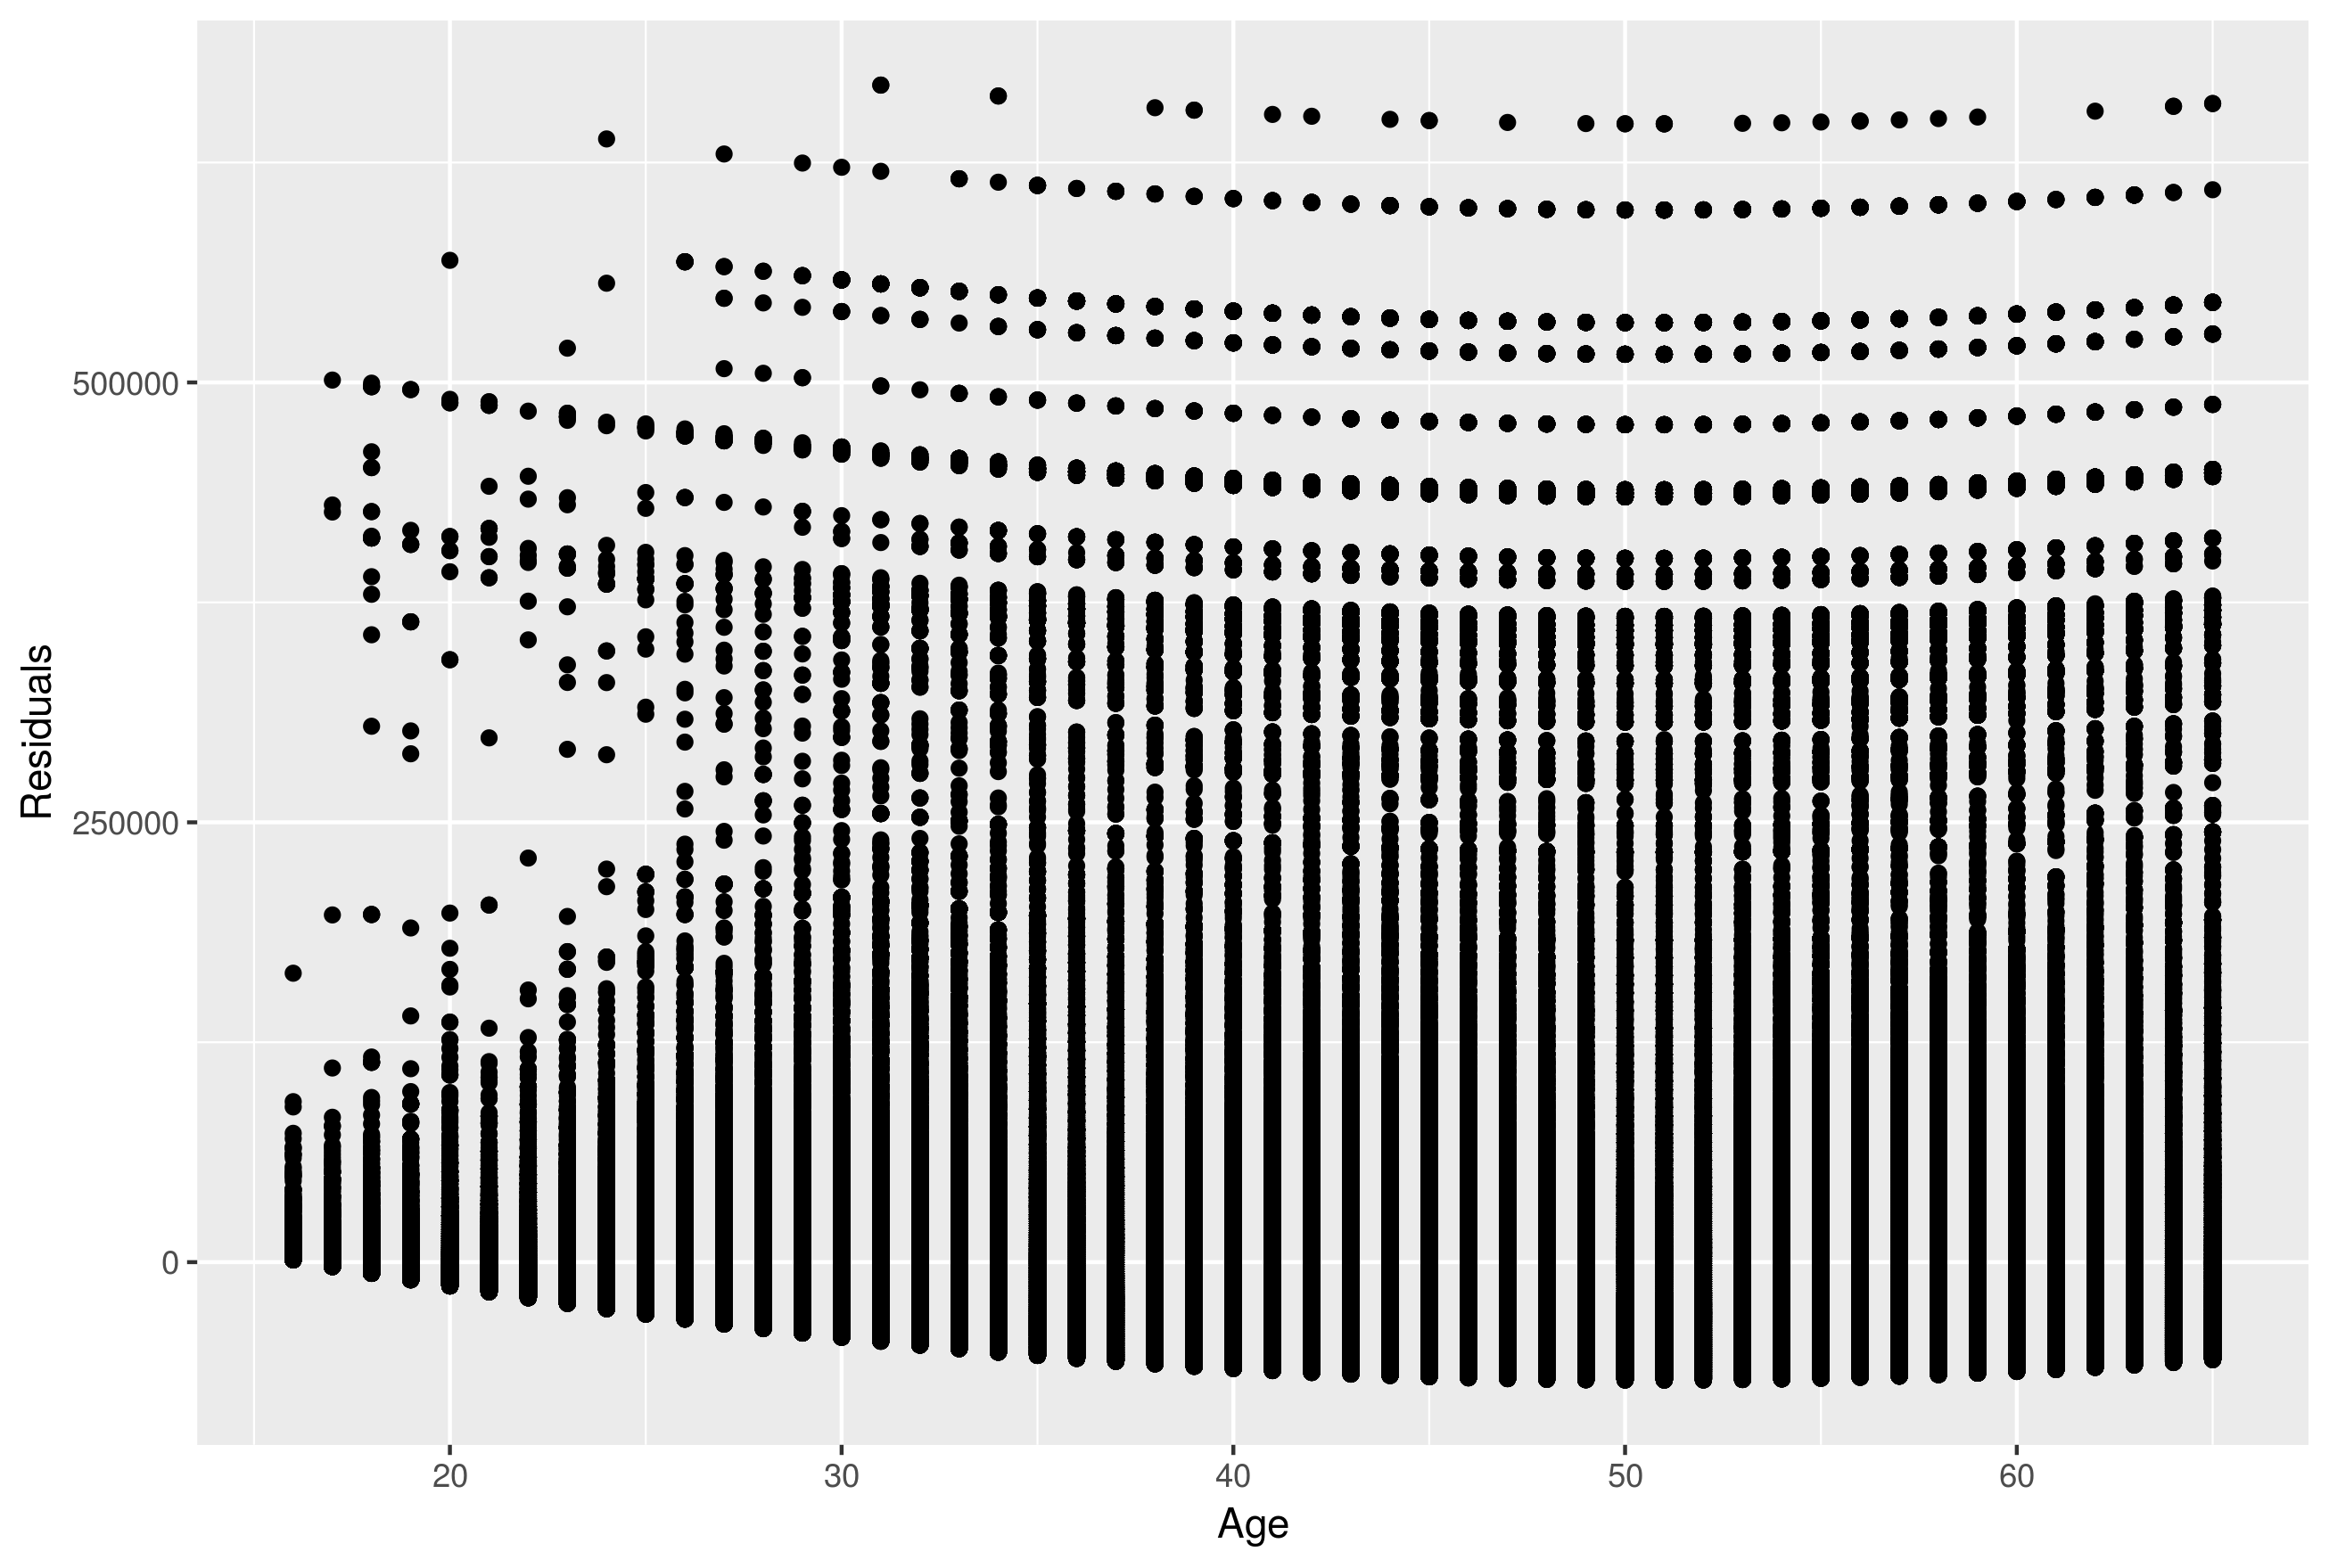
\includegraphics[width=90mm]{residuals.png}
\caption{Residuals vs Age \label{overflow}}
\end{figure}


\item Obtain robust standard errors in R and Stata. (18 points)

The values of the robust standard errors found in R were as follows:\\
With no adjustment for degrees of freedom:

Age:  23.6251\\
Age2:  0.3024647\\
Cons:  399.5719148\\

We adjusted these values for the degrees of freedom using:

$ N/(N-k)$

Age:  23.625128\\
Age2:  0.302465 \\
Cons:  399.572365\\

Using Stata we found the following values for robust standard errors:

Age:  23.62513\\
Age2:  0.302465 \\
Cons:  399.5724\\

\end{enumerate}
\end{document}

